\documentclass{article}
\usepackage{hyperref}
\usepackage{csquotes}
\usepackage[vmargin=25mm, hmargin=20mm]{geometry}
\usepackage{longtable}
\usepackage{array}
\usepackage[style=ieee, maxcitenames=2, mincitenames=1]{biblatex}
\addbibresource{sources.bib}
\usepackage{multicol}
\usepackage{float}
\usepackage{graphicx}

\title{Looking at Challenges and Mitigation in Symbolic Execution Based Fuzzing Through the Lens of Survey Papers}
\author{Valentin Huber}
\begin{document}
% ----------
% FORMATTING 
% ----------

% Bullet list vertical spacing
\let\savedItemize=\itemize
\let\savedEndItemize=\enditemize
\renewenvironment{itemize}{\savedItemize\setlength\itemsep{0px}}{\savedEndItemize}

% Make Tables less crowded
\AtBeginEnvironment{longtable}{\renewcommand\arraystretch{1.6}}
\newcolumntype{P}[1]{>{\raggedright\arraybackslash}p{#1}}

% Column separation
\setlength{\columnsep}{13mm}

% Font size for bibliography
\renewcommand*{\bibfont}{\footnotesize}

% introduce non-breaking space before citations and references
\let\savedCite=\cite
\renewcommand{\cite}{\unskip~\savedCite}
\let\savedRef=\ref
\renewcommand{\ref}{\unskip~\savedRef}

% --------
% WARNINGS
% --------

% Disable minimally overfull hbox warnings
\hfuzz=50px

% Disable minimally underfull hbox warnings
\hbadness=1000

% ---------------
% CUSTOM COMMANDS
% ---------------

\newcommand{\tableh}[1]{\multicolumn{1}{|c|}{\textbf{#1}}} % table header
\newcommand{\code}{\texttt}
\newcommand{\papertitle}[1]{\citetitle{#1} (\citedate{#1})\cite{#1}}

\maketitle
\begin{multicols}{2}
    \tableofcontents

    \section{Introduction}
    In 2022, the cost of poor software quality was estimated to be more than \$2.4 trillion in the US alone.\cite{CostPoorSoftware} Individual cyber attacks have had an estimated financial impact of up to \$8 billion worldwide.\cite{Demystifying} Testing software often accounts for more than 50\% of development costs\cite{Orchestrated}, but it is typically a mostly manual process\cite{PreliminaryAssessment}. Because manual testing requires many developer hours with in-depth knowledge of the system being tested, it does not scale well. Automated testing promises to be more cost effective in finding software defects and has therefore become the most popular vulnerability discovery solution, especially in the industry.\cite{FuzzingASurvey}

    One such automated vulnerability and bug testing technique is fuzzing.\cite{VulnerabilityDiscoveryTechniques} In the seminal work by \citeauthor{UNIX} in \citeyear{UNIX}, the term \textquote{fuzz} is defined as a program that \textquote{generates a stream of random characters to be consumed by a target program}\cite{UNIX}. Since then, a rich ecosystem of fuzzing systems has emerged in both industry and academia, taking design inspiration from a wide variety of software engineering concepts. These are combined into programs that generate various concrete inputs, which are then repeatedly fed into a particular program under test (PUT), and check the program for illegal states or crashes.\cite{EvaluatingFuzzTesting}

    Fuzzing is widely used in industry, with major technology companies and government agencies such as Google, Microsoft, the US Department of Defense, Cisco and Adobe developing proprietary fuzzers and contributing to open source fuzzers. These are then used to great effect, with Google alone finding 20,000 vulnerabilities in Chrome alone using fuzz testing.\cite{Demystifying}

    Another approach to automated software testing is symbolic execution\cite{Symbex}. Test frameworks based on symbolic execution do not run programs with concrete inputs, but with variables representing all possible values. By tracking how these values are used, systems based on pure symbolic execution can then reason about and even prove certain hypotheses in a PUT. However, because these systems must essentially emulate the entire program, including all possible program states, pure symbolic execution only works on trivial programs, and breaks down on real-world programs because of their size. Naïve implementations further cannot handle non-trivial software that may be multi-threaded or interact with its environment.

    Over the past decades, many fuzzers\cite{BitBlaze,CORAL,CREST,CUTE,CVC5,CVCLite,Chopped,Cyberdyne,DART,DTSA,DiSE,DigFuzz,Dowser,Driller,EGT,EXE,Fitnex,FloPSy,GRT,GSE,HCT,HFL,IFL,Intriguer,JFI,KATCH,KLEE,KLEEFP,LATEST,MoWF,Moles,PYGMALION,Pangolin,Pex,QSYM,QuickFuzz,RWset,SAGE,SAVIOR,SMART,SPIN,STP,ScalableAutomatedMethods,TFuzz,TaintScope,VUzzer} have employed symbolic execution based techniques, with great success: SAGE\cite{SAGE} \textquote{reportedly found a third of the Windows 7 bugs between 2007-2009}\cite{FuzzingTheStateOfTheArt}.

    Since the academic research in this area is vast, existing reviews are used to filter the work on the topic at hand to the most important. The following contributions are made on this basis:

    \begin{itemize}
        \item First, the theoretical principles behind fuzzing and symbolic execution are explained in Section\ref{Theory}.
        \item Second, Section\ref{Methods} explains the reasoning behind using existing survey papers to base this work on.
        \item Third, an overview of existing survey papers investigating the state of fuzzing is given in Section\ref{SurveyPapers}, along with a short summary of each paper.
        \item Fourth, the challenges fuzzing tools face in implementing symbolic execution techniques, and attempts to mitigate each of them, are listed along with examples of works that implement them in Section\ref{Results}.
        \item Finally, limitations and possible additions to this work are discussed in Section\ref{Discussion}.
    \end{itemize}

    \section{Theoretical Principles}
    \label{Theory}

    To understand the limitations of symbolic execution and innovations introduced in papers, a fundamental understanding of both general fuzzing procedures and symbolic execution is crucial.

    \subsection{Fuzzing}

    \citeauthor{UNIX} in \citeyear{UNIX} both invented the term and laid the foundation for fuzzing. They observed that, during a stormy night, lightning strikes would introduce interference in their dial-up based communication channel to a UNIX system, which changed the intended inputs and crashed the tools they were using. They then attempted to reproduce this systematically by repeatedly running tools with random inputs containing a combination of printable, non-printable and \code{NULL} bytes. On different UNIX systems, they were able to crash between 25 and 30\% of all tested utility programs.\cite{UNIX}

    \begin{figure*}[!tp]
        \centering
        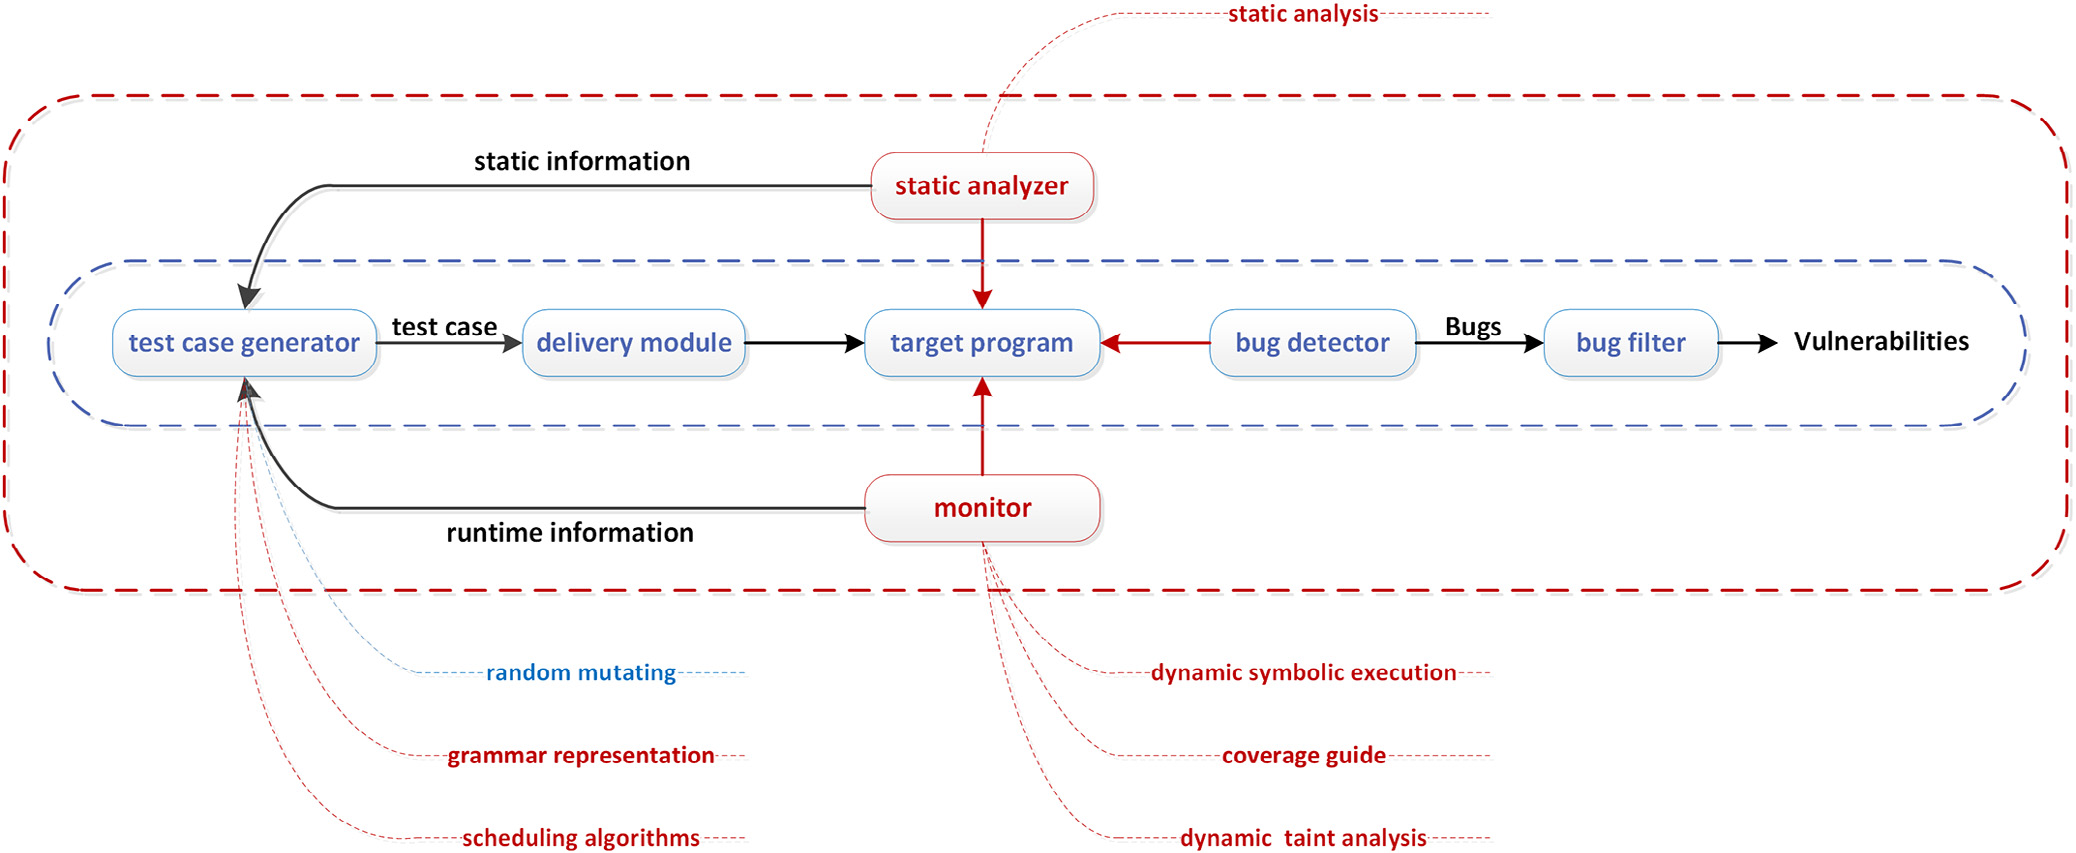
\includegraphics[width=0.9\textwidth]{assets/FuzzingSteps.jpg}
        \caption{Architectural Diagram of a Fuzzing System\cite{Science}}
        \label{fig:FuzzingSteps}
    \end{figure*}

    \subsubsection{Similarities Across Fuzzers}
    Ever since then, these fuzzing systems have become more sophisticated and different techniques have been integrated. However, certain characteristics remain similar between all fuzzing systems. They output some concrete input(s) and configurations that can then be used to reproduce the fuzzer's observation, allowing confirmation, reproduction, and debugging of the discovered issues.\cite{EvaluatingFuzzTesting} They automatically find well-defined bugs, such as assertion errors, divisions by zero, \code{NULL} pointer dereferences, etc.\cite{AllYouEverWanted}

    \subsubsection{Architecture of a Fuzzer}
    \label{ArchitectureFuzzer}
    Figure\ref{fig:FuzzingSteps} shows the architecture of a typical fuzzer. Most fuzzers contain similar parts responsible for each step during the fuzzing process. These are explained below

    \paragraph{Target Program}
    The target program (also known as the program under test, or PUT) is the software to be tested. Different fuzzers have different requirements for the kind of PUT they support: Some require access to source code to add instrumentation during the compilation or because they work on a intermediate representation (IR), such as LLVM bytecode.

    \paragraph{Bug Detector}
    The bug detector observes the PUT during execution for illegal states. The simplest implementations trigger on program crashes, more sophisticated bug detectors might check if certain protected parts of the PUT are accessed, for example to check the authentication implemented.

    \paragraph{Bug Filter}
    The list of inputs that put a PUT into an illegal state may contain duplicates, in a sense that the exploit the same software defect. The bug filter attempts to deduplicate this list based on some heuristics like the order basic blocks were executed in or stack hashes.

    \paragraph{Test Case Generator}
    The test case generator's job is to generate and select the next input to be tested. Based on the test case generator, fuzzing systems can be categorized as either mutation-based or generation-based. Mutation-based fuzzers take some input to the PUT as their input, and then repeatedly mutate those if the results produce \textquote{interesting} behavior\cite{EvaluatingFuzzTesting}.

    The prioritization is either done randomly or based on some heuristic, which assign each possible next input a value used to select the next input to be passed to the delivery module. Heuristics often take into account information produced by the monitor like coverage or distance to target instructions. These approaches can further be combined, e.g. by alternating random and heuristic-based input selection.

    \paragraph{Delivery Module}
    The delivery module is responsible to pass the generated test case to the PUT in the expected form and trigger the actual execution. This might be as simple as starting a command line utility with certain command line arguments, but might also include creating files that are accessed by the PUT or even emulating user interaction.

    \paragraph{Monitor}
    Fuzzing systems can further be classified based on how much access the monitor module has to the PUT. Blackbox fuzzers make a single observation: whether or not the PUT crashed. Graybox fuzzers have limited access to the PUT during execution. Typical information extracted by graybox fuzzers includes which basic blocks were executed in what order, or generally code coverage based on instruction, basic block, or statement. Whitebox fuzzers have full access to the PUT and allow for sophisticated reasoning about the program structure. Systems that employ taint analysis or symbolic execution are categorized as whitebox fuzzers, since they deeply examine the program structure during their analysis. Different systems make different tradeoffs, accepting higher analysis cost, in the hope of better bug-finding effectiveness.\cite{EvaluatingFuzzTesting}

    \paragraph{Static Analyizer}
    The static analyzer, as its name suggests, attempts to extract information by statically examining the PUT's source code, IR or binary. Such information might include grammars accepted by the PUT or program paths deemed high-risk.

    \subsection{Symbolic Execution}
    The concept of symbolic execution in the context of program testing was introduced in \citeyear{Symbex} by \citeauthor{Symbex}.\cite{Symbex} By not executing a PUT with concrete values (such as the number \code{23} or the string \code{"Hello World!"}) but instead modelling certain or all values with mathematical variables, it allows exploring all possible paths of a program. Different engines (such as angr\cite{angr} or Triton\cite{Triton}) allow performing symbolic execution on source code, an IR, or a binary of a PUT.

    \subsubsection{Performing Symbolic Execution}
    During execution of a certain program, with each instruction a symbolic execution engine computes and updates the so-called symbolic state. It contains:
    \begin{itemize}
        \item the inputs marked as symbolic as symbols $\alpha_i$,
        \item the symbolic expression store $\sigma$, which in turn contains
        \item symbolic expressions $\phi_j$, which are either a reference to a symbol $\alpha_i$, or an arithmetic combination of symbolic expressions, such as $\phi_j=\phi_k-\phi_l$, and finally
        \item the path constraint $\pi$, which is the conjunction of all branch constraints, which are the conditions on symbolic expressions to end up at a certain point in the program, such as $\phi_1\leq2$ or $\phi_2=\phi_3\land\phi_4=3$.
    \end{itemize}

    During execution, the symbolic state is changed according to the specific instruction currently executed. If it performs some form of manipulation on existing data, this is represented by adding new symbolic expressions to the symbolic store. If a branch is (not) taken based on a check on variables or registers containing symbolic expressions, the path constraint is extended with an appropriate condition. The exploration of a program can follow different heuristics, such as breath- or depth-first search.

    \subsubsection{Categorizing Symbolic Execution Implementations}
    Symbolic execution implementations can be categorized in several ways: Where static dynamic execution exclusively and exhaustively performs the process described above, dynamic (or concolic, a portmanteau of \textquote{concrete} and \textquote{symbolic}) symbolic execution executes a program symbolically and with concrete values in parallel.

    Online symbolic execution allows calculating multiple paths in parallel, while offline symbolic execution examines one path after the other. Finally, one can distinguish between partial and full symbolic execution, where only a part, or all the variable, and therefore calculation is done symbolically.\cite{Ghidrion}

    \section{Methods}
    \label{Methods}
    Fuzzing is an extensively researched topic. For the search term \textquote{Fuzzing}, Web of Science\cite{WebOfScience} finds 2,741, Scopus\cite{Scopus} 2,410, and Google Scholar\cite{GoogleScholar} approximately 29,300 works. Even when filtered by top venues, to summarize the current state of symbolic execution in fuzzing would be a task beyond what is feasible in this project.

    However, since fuzzing is such a well-published topic, other researchers have taken on the work of summarizing the state of the art, each group with a slightly different focus. These survey papers can therefore be used to approximate a complete picture of the current state of the art. This is the approach chosen by the author of this paper. Section\ref{SurveyPapers} contains a list of survey papers taken into consideration. To ensure accuracy and a consistent level of detail, works discussed in these review papers (primary works) are used to corroborate or refute how review papers discuss the contributions of each primary work.

    To select review papers to consider, the following rules were applied:
    \begin{itemize}
        \item First, different search engines were used to create a list of survey papers in the field of fuzzing. Since even the amount of survey papers is overwhelming (Google Scholar\cite{GoogleScholar} returns more than 25,000 results for the search term \textquote{fuzzing survey}), works were only included if their title, abstract, or keywords contained the word section \textquote{fuzz} and if Google Scholar\cite{GoogleScholar} reports that they were cited more than 5 times or if they were published in a high-impact venue.
        \item Then, further review papers discussed, listed, or cited in other review papers were added (such as works listed in \cite{Demystifying}).
        \item Works published before January 1, 2010 (such as\cite{ViolatingAssumptionsWithFuzzing} or\cite{NewTrendsSymbex}) were disregarded to further limit the scope of this survey.
        \item Then, review papers focusing on a specific technique (such as machine learning\cite{ML1, ML2}) were disregarded.
        \item Additionally, works focusing on a specific use case for fuzzing, such as testing internet of things or other embedded devices\cite{IoT, Embedded, Embedded2}, network protocols\cite{Network, Network2023}, smart contracts\cite{Ethereum}, or JavaScript engines\cite{JavaScript, JavaScript2} were disregarded.
        \item Finally, a selection of additional works were added to the list based on the author's intuition.
    \end{itemize}

    \section{Related Work}
    \label{SurveyPapers}

    This section summarizes contributions of existing survey papers selected as described in Section\ref{Methods} and lists relevant primary works discussed in each. Primary works mentioned without discussion are omitted.

    \papertitle{AllYouEverWanted}
    Using a simple intermediate language (SIMPIL), this paper discusses taint analysis and forward symbolic execution, including examples and analysis of the theoretical foundations of symbolic execution. While fuzzing is mentioned in multiple instances, it is not the main focus. However, it still lists many of the drawbacks and advantages fuzzers based on symbolic execution have, and the additional perspective was valuable in assembling this review.

    \papertitle{PreliminaryAssessment}
    After giving a short overview of issues faced by symbolic execution based fuzzers, this paper focuses on eight high impact fuzzing tools (JPF-SE and Symbolic (Java) PathFinder\cite{JPFSE, JavaPathFinder}, DART\cite{DART}, CUTE\cite{CUTE} and jCUTE\cite{ExplicitPathModelChecking}, CREST\cite{CREST}, SAGE\cite{SAGE}, Pex\cite{Pex}, EXE\cite{EXE}, and KLEE\cite{KLEE}).

    \papertitle{Orchestrated}
    Orchestrated surveys \textquote{consist of a collaborative work collecting self-standing sections, each focusing on a key surveyed topic}\cite{Orchestrated}. One of the topics discussed in this particular work is symbolic execution. It contains short introductions into BBRBP\cite{BBRBP}, AGLT\cite{AGLT}, Darwin\cite{Darwin}, MATRIX RELOADED\cite{MATRIXRELOADED}, and SRA\cite{SRA} in its introduction. As mitigation strategies for path explosion, it discusses SMART\cite{SMART}, DDCSE\cite{DDCSE}, PFA\cite{PFA}, among others. For environment interaction, ASSIE\cite{ASSIE} and Cinger\cite{Cinger} are presented. Finally, to attempt to solve constraints that are too complex for direct SMT solver invocation, MCSS\cite{MCSS}, CORAL\cite{CORAL}, and its extension introducing AVM\cite{CORALAVM} are cited.

    \papertitle{FuzzingTheStateOfTheArt}
    \citeauthor{FuzzingTheStateOfTheArt} from Australia's Department of Defence provide an extensive look at fuzzing — \citetitle{FuzzingTheStateOfTheArt} is the longest of the discussed survey papers. After discussing the taxonomy, concepts, types, and history of fuzzing, they discuss a list of 15 works from scientific literature and ten commercial and open-source frameworks. In those scientific works, they present four papers that employ symbolic execution, namely KLEE\cite{KLEE}, SAGE\cite{SAGE}, GWF\cite{GWF}, and TaintScope\cite{TaintScope}.

    \papertitle{ReviewThreeDecades}
    This survey paper, as the title suggests, focuses on symbolic execution. Starting with an explanation of classical symbolic execution, it then provides a list of issues that fuzzing tools based on symbolic execution face, along with attempts to mitigate those by adapting and extending the algorithms. Finally, the authors present five high-impact tools they worked on: DART\cite{DART}, CUTE\cite{CUTE}, CREST\cite{CREST}, EXE\cite{EXE}, and KLEE\cite{KLEE}.

    \papertitle{Science}
    After discussing the structure of fuzzing systems and different targets observed in literature and industry, this paper focuses on inventions of primary works along the structure of fuzzers. Symbolic execution is discussed in the context of the sample generator and the monitor (see Section\ref{ArchitectureFuzzer}). Discussed primary works include CUTE\cite{CUTE}, KLEE\cite{KLEE}, SAGE\cite{SAGE}, TaintScope\cite{TaintScope}, BuzzFuzz\cite{BuzzFuzz}, GWF\cite{GWF}, Dowser\cite{Dowser}, BORG\cite{BORG}, Driller\cite{Driller}, and MoWF\cite{MoWF}. It further contains a sizeable section comparing symbolic execution based fuzzing systems and their contributions.

    \papertitle{FuzzingASurvey}
    \citeauthor{FuzzingASurvey} focus on coverage-guided fuzzing, mentioning other approaches that can be mixed in and different applications it can be used for. They further broadly discuss the challenges symbolic execution in fuzzing faces. Last, they present TaintScope\cite{TaintScope} and Driller\cite{Driller} as examples of using symbolic execution for specifically for path exploration.

    \papertitle{FuzzingStateOfTheArt2018}
    The first mention of a symbolic execution based fuzzer in this paper is SAGE\cite{SAGE}, which the authors use to summarize the limitations of whitebox fuzzing. In the following section, works bringing progress to a step in the fuzzing workflow are discussed, including SYMFUZZ\cite{SYMFUZZ}, TaintScope\cite{TaintScope} and KATCH\cite{KATCH}. Then, and most clearly relevant for this work, \citetitle{FuzzingStateOfTheArt2018} contains a discussion of the limitations of taint analysis and dynamic symbolic execution. Discussed works in this section include, among others,  SMART\cite{SMART}, HOTG\cite{HigherOrderTestGeneration}, Cloud9\cite{Cloud9}, APLS\cite{APLS}, SAGE\cite{SAGE}, CGF\cite{CGF}, DeepFuzz\cite{DeepFuzz}, TCR\cite{TCR}, DiSE\cite{DiSE}, and CRAXfuzz\cite{CRAXfuzz}.

    \papertitle{EvaluatingFuzzTesting}
    While not a classic survey paper, \citetitle{EvaluatingFuzzTesting} finds issues in how all 32 papers performed the evaluation of the system they introduced. It further proposes rules to follow to make an evaluation robust. Last, it contains a list of what advances each paper examined claims to introduce.

    \papertitle{ArtScienceEng}
    Starting with proposing a taxonomy for fuzzing itself and categorizing fuzzers, this paper proposes a general-purpose model of fuzzing, explaining the steps and approaches common fuzzers share. It further presents a genealogy, tracing the origins of important papers back to the work of \citeauthor{UNIX}. However, it \textquote{does not provide a comprehensive survey on DSE}\cite{ArtScienceEng}, but only discusses whitebox fuzzing in a subsection and refers to other survey papers such as \cite{Orchestrated, AllYouEverWanted} for a more complete overview.

    \papertitle{FuzzingASurveyforRoadmap}
    Similar to what is attempted in this paper, \citetitle{FuzzingASurveyforRoadmap} lists issues along common steps in fuzzing along with attempted solutions, but without the focus on symbolic execution. It does contain a short section about symbolic execution in the context input search space handling, but only discusses very few papers directly while often mentioning entire families of papers, with only some relying on symbolic execution.

    \papertitle{FuzzingVulnerabilityDiscoveryTechniques}
    After a short chapter on fuzzer classification, the main focus of this paper are steps and issues along a typical fuzzer workflow, told through the papers that made advances in each category. Finally, it presents current challenges in research and how they could be approached. The discussed papers include some that rely on symbolic execution: Angora\cite{Angora}, T-FUZZ\cite{TFuzz}, MoWF\cite{MoWF}, and HFL\cite{HFL}.

    \papertitle{SystematicReview2023}
    The authors of this paper guide the reader through advances in fuzzing along the works that introduced those. It includes a section about symbolic execution, which considers the following systems: Driller\cite{Driller}, QSYM\cite{QSYM}, SAVIOR\cite{SAVIOR}, DigFuzz\cite{DigFuzz}, Pangolin\cite{Pangolin}, and QuickFuzz\cite{QuickFuzz}.

    \papertitle{Demystifying}
    This paper dedicates one of its chapter to first explaining the fundamental logic of symbolic execution, and then presenting three implementations (Driller\cite{Driller}, CONFETTI\cite{CONFETTI}, and FUZZOLIC\cite{FUZZOLIC}). It further investigates advances in IoT firmware and kernel fuzzers, but does not explain where up- and downsides of using symbolic execution in these domains lay.

    \subsection{TODO}
    \begin{itemize}
        \item    Fuzzing: hack, art, and science (\citedate{HackArtScience})\cite{HackArtScience}
        \item    A Survey of Hybrid Fuzzing based on Symbolic Execution (\citedate{SurveyHybrid})\cite{SurveyHybrid}
        \item    Fuzzing: Challenges and Reflections (\citedate{ChallengesAndReflections})\cite{ChallengesAndReflections}
        \item    Exploratory Review of Hybrid Fuzzing for Automated Vulnerability Detection (\citedate{Hybrid})\cite{Hybrid}
    \end{itemize}

    \section{Challenges and Mitigation}
    \label{Results}
    Heavily based on \cite{ReviewThreeDecades, PreliminaryAssessment}, extended based on information from all other information considered as listed in Section\ref{SurveyPapers}.

    This section focuses on attempts to mitigate inherent issues with symbolic execution. Many of the listed papers implemented further more general efficiency improvements, like SAGE's\cite{SAGE} (and multiple other papers inspired by it) generational search, which generates multiple new inputs from just one run of the symbolic execution engine by solving the constraint formula with the constraint from each branch flipped independently.

    \subsection{Impossible Constraints}
    \begin{itemize}
        \item \textquote{A key disadvantage of classical symbolic execution is that it cannot generate an input if the symbolic path constraint along a feasible execution path contains formulas that cannot be (efficiently) solved by a constraint solver (for example, nonlinear constraints).}\cite{ReviewThreeDecades}
        \item Two techniques that alleviate this problem:
              \begin{itemize}
                  \item Dynamic Symbolic Execution (DSE), or Concolic Testing (like DART\cite{DART} and its successor CUTE\cite{CUTE}, and CREST\cite{CREST}): Run concrete and symbolic execution at the same time, keep mapping between values, solve path constraint with one sub-constraint flipped to get input for an other path. \textquote{A key observation in DART is that imprecision in symbolic execution can be alleviated using concrete values and randomization}\cite{PreliminaryAssessment}
                  \item Execution-Generated Testing (EGT)\cite{EGT} (like EXE\cite{EXE} and KLEE\cite{KLEE}): Only execute symbolically if any operands are symbolic
              \end{itemize}
        \item These handle imprecision in symbex (like interaction with outside code (that is not instrumented for symbex), constraint solving timeouts, unhandled instructions (floating point), or system calls (\code{read}, interrupts, etc.)) by just using concrete values.
              \begin{itemize}
                  \item If none of the operands are symbolically, just use them
                  \item If any are, use the concrete values (direct in concolic, solution from path constraint in EGT)
              \end{itemize}
        \item Downside: missing some feasible paths, and therefore sacrificing completeness.
        \item Further Ideas: Special Constraint Solvers that improve floating point based constraint handling (like FloPSy\cite{FloPSy}) and complex mathematical constraints (like CORAL\cite{CORAL} and its extension\cite{CORALAVM})
    \end{itemize}

    \subsection{System Calls}
    \begin{itemize}
        \item \textquote{Additionally, symbolic execution creates conflicts while handling system calls, since it does not support modeling all possible system calls and inter-process communication, such as pipes or sockets. Likewise, the non-deterministic behavior of system calls complicates the generation of inputs that consistently trigger specific paths.}\cite{Demystifying}
        \item HFL\cite{HFL} is a kernel fuzzer that heavily relies on symbolic execution. It lists three main issues the authors had to overcome: \textquote{(1) indirect control transfers determined by system call arguments (2) controlling and matching internal system state via system calls, and (3) nested argument type inference for invoking system calls}\cite{HFL}. To solve those issues, HFL \textquote{(1) converts implicit control transfers to explicit transfers, (2) infers system call sequence to build a consistent system state, and (3) identifies nested arguments types of system calls}\cite{HFL}.
    \end{itemize}

    \subsection{Environment Interaction}
    \begin{itemize}
        \item \textquote{[…KLEE's\cite{KLEE}] ability to handle interactions with the outside environment — e.g., with data read from the file system or over the network — by providing models designed to explore all possible legal interactions with the outside world.}\cite{PreliminaryAssessment}
        \item The path constraints per instruction can also be generated automatically, like in ASSIE\cite{ASSIE}.
        \item Further automation allows Cinger\cite{Cinger} to analyze a PUT and prompt the user to present models only for the program parts that actually introduce imprecision.
    \end{itemize}

    \subsection{Path Explosion}
    Path Explosion: program path count usually exponential in the number of static branches in the code.
    \begin{itemize}
        \item Simple depth-first search, however this naïve approach gets stuck in non-terminating loops with symbolic conditions and is therefore rarely used. Both EXE\cite{EXE} and KLEE\cite{KLEE} can however be configured to run in this mode.
        \item Symbex inherently helps by only looking at possible branches. Example: EXE\cite{EXE} on \code{tcpdump}: only 42\% of instructions contained symbolic operands, less than 20\% of of symbolic branches have both sides feasible\cite{EXE}
        \item Prioritization of which path to explore next using heuristics (like statement or branch coverage (and using static analysis to guide), favouring statements that were run the fewest number of times, or random). Examples: EXE\cite{EXE}, SAGE\cite{SAGE}, CREST\cite{CREST}
              \begin{itemize}
                  \item \textquote{CREST\cite{CREST} is an extensible platform for building and experimenting with heuristics for selecting which paths to explore}\cite{ReviewThreeDecades}, allows implementing heuristics based on static analysis, namely control flow graphs.
                  \item Prioritize inputs that increase path coverage the most, as implemented in many fuzzers, including SAGE\cite{SAGE}
                  \item Interleave random and symbolic execution. Examples: Hybrid Concolic Testing\cite{HCT, Driller, Cyberdyne}
                  \item Guide towards changes in a patch: Directed Incremental Symbolic Execution\cite{DiSE}, Directed Test Suite Augmentation\cite{DTSA}, MATRIX RELOADED\cite{MATRIXRELOADED}, and KATCH\cite{KATCH}, which is based on KLEE\cite{KLEE}.
                  \item Guide towards interesting function calls, such as \code{malloc}, as in CRAXfuzz\cite{CRAXfuzz}
                  \item Reward inputs that lead to longer runtime, as in AGLT\cite{AGLT}, or those that produce vastly different outputs based on very similar inputs, as in SRA\cite{SRA}.
                  \item Chopped symbolic execution ignores (resp. only lazily executes) certain functions deemed uninteresting to focus on certain parts of the PUT and prevent path explosion. This can either be done manually or automatically based on some heuristics (like code unassociated with changes in a patch in Chopper\cite{Chopped}).
                  \item \textquote{we propose a novel approach called Fitnex, a search strategy that uses state-dependent fitness values (computed through a fitness function) to guide path exploration. The fitness function measures how close an already discovered feasible path is to a particular test target (e.g., covering a not-yet-covered branch)}\cite{Fitnex}
                  \item Weigh the approximate cost of executing a certain path against its demand, as done in QuickFuzz\cite{QuickFuzz}
                  \item Assign probabilities to execution paths to reach deeper execution, as in DeepFuzz\cite{DeepFuzz}
                  \item Probabilistic approach: Use Monte Carlo path optimization to quantify the difficulty of each path using grey-box fuzzing to then let the white-box fuzzer focus on the paths that are believed to be most challenging for grey-box fuzzing to make progress.\cite{DigFuzz}
                  \item Guide execution towards code parts deemed to be interesting based on static analysis, such as pointer dereferences in loops as implemented in Dowser\cite{Dowser}, potential bugs according to UndefinedBehaviorSanitizer\cite{UndefinedBehaviorSanitizer} in SAVIOR\cite{SAVIOR}, buffer over-reads in BORG\cite{BORG} or more general prior static or dynamic program analysis such as in GRT\cite{GRT} or VUzzer\cite{VUzzer} to guide the symbolic execution engine.
              \end{itemize}
        \item Pruning redundant paths (\textquote{if a program path reaches the same program point with the same symbolic constraints as a previously explored path, then this path will continue to execute exactly the same from that point on and thus can be discarded.}\cite{RWset}) Eliminating redundant paths by analyzing the values read and written by the program.
        \item Similarly, MoWF\cite{MoWF} uses knowledge gained by its built-in blackbox fuzzer to prune invalid inputs and thus prevents its symbolic execution engine to get stuck in input checking and error handling code. CESE\cite{CESE} uses context-free grammars to limit its symbolic execution engine to interesting paths, as opposed to error handling during parsing. TCR\cite{TCR} intelligently reduces existing test cases and prioritizes the remaining according to heuristics to maximize exploration efficiency.
        \item State-merging to reduce the number of states in memory, as in KLEE\cite{KLEE}, Mayhem\cite{Mayhem}, S2E\cite{S2E}, BORG\cite{BORG}, and Cloud9\cite{Cloud9}
        \item Sharing among states/copy on write: KLEE\cite{KLEE}
        \item Transfer state from memory to disk, as in Mayhem\cite{Mayhem}, BORG\cite{BORG}, and SAGE\cite{SAGE}
        \item Caching function summaries for later use by higher-level functions. These can be generated automatically, like in SMART\cite{SMART}, HOTG\cite{HigherOrderTestGeneration}, or DDCSE\cite{DDCSE}, or manually, like in PFA\cite{PFA}.
        \item Similarly, common complex structures like strings and regular expressions can be manually transformed into constraints. An example of this would be PFA\cite{PFA}.
        \item Lazy test generation (as in LATEST\cite{LATEST})
        \item Static path merging (as in KLEE-FP\cite{KLEEFP})
        \item partial order and symmetry reductions (as in GSE\cite{GSE})
        \item Compact representation of path constraints (as in SAGE\cite{SAGE})
    \end{itemize}

    \subsection{Constraint Solving}
    \label{ConstraintSolving}
    Dominates runtime
    \begin{itemize}
        \item Irrelevant constraint elimination: Generally, we go from a solvable constraint set (namely the current execution with the solution being the current concrete values) to one where only one constraint changes (the one we flipped). Typically, major major parts of the constraint set are not influenced by the change and can be excluded from what is passed to the solver. We can then just use the values from the previous iteration. This is implemented, among others, in \cite{SAGE}.
        \item Concolic/dynamic symbolic execution, use concrete values, as in DART\cite{DART} or CUTE\cite{CUTE}.
        \item Similarly, if the whole constraint is not solvable, solve parts of it and use those concrete values to solve the rest, as in MCSS\cite{MCSS}.
        \item Identify independent sub-queries and solve them independently, as is done in EXE\cite{EXE} and KLEE\cite{KLEE}.
        \item \textquote{loop-guard pattern matching rules to identify a constraint that defines the number of iterations of input-dependent loops during dynamic symbolic execution, then set new constraints representing the pre- and post-loop conditions to summarize sets of executions of that loop}\cite{Science}, as in SAGE\cite{SAGE}, BORG\cite{BORG}, and APLS\cite{APLS}
        \item Optimizing SMT queries before passing them to the solver. The optimization itself, however, can already be too complex to compute to employ this strategy effectively.
        \item Mocking and stubbing: Moles\cite{Moles}
        \item Incremental solving: Reuse the results of previous similar queries, because subsets of the constraints are still solved by the same results and supersets often do not invalidate existing solutions. (CUTE\cite{CUTE} and counterexample caching scheme in KLEE\cite{KLEE})
        \item Cache prior SMT query results and reuse them for future queries. Pangolin\cite{Pangolin} uses polyhedral path abstraction to replace query parts for more efficient models based on prior results.
        \item Improved SMT solvers (like Z3\cite{Z3} used in e.g. SAGE\cite{SAGE}, STP\cite{STP}, Yices\cite{Yices}, or cvc5\cite{CVC5} built during the development of EXE\cite{EXE})
        \item Intriguer\cite{Intriguer} uses taint analysis to discover instructions accessing a wide range of input bytes, and then performs symbolic execution for those instructions deemed important and only invoke the underlying SMT solver for complicated queries.
        \item SMT formulas can be transformed into programs, which in turn can then be solved using a coverage-guided fuzzer to generate solutions to the initial formula. JFI\cite{JFI} uses this technique to find solutions to floating-point constraints.
        \item Do not use intermediate representation (IR) to execute symbolically, but integrate the symbolic emulation with the native execution through dynamic binary translation, which prevents additional instructions (since often multiple RISC instructions are necessary to replace one CISC instruction), and allows finer-grained control over the constraint, thus making it smaller. Example: QSYM\cite{QSYM}
        \item While technically not using symbolic execution, analyzing the dependency between input data and state space and approximating solutions to path constraints based on those to prevent expensive calls to an SMT solver is fairly common\cite{WEIZZ}:
              \begin{itemize}
                  \item Eclipser\cite{Eclipser} uses instrumentation on the PUT to generate partial path conditions, which can then be solved without invoking SMT solvers to generate further inputs.
                  \item Angora\cite{Angora} uses solves path constraints by using a combination of context-sensitive branch coverage, scalable byte-level taint tracking, gradient descent searching, input length exploration, and type and shape inference.
                  \item REDQUEEN\cite{REDQUEEN} exploits the fact that much of the input data ends up in the state-space and uses simple transformations on the input data as opposed to relying on taint analysis or symbolic execution to bypass checksums.
                  \item Other proposals include approximate SMT solvers, such as FUZZY-SAT implemented in FUZZOLOGIC\cite{FUZZOLIC}, or optimistic SMT solvers, as in QSYM\cite{QSYM}.
              \end{itemize}
    \end{itemize}

    \subsection{Modelling}
    Things like modelling \code{int}s as mathematical integers being imprecise since it ignores over-/underflows, and pointers being hard to deal with.
    \begin{itemize}
        \item Issue: Dereferencing symbolic pointer, as in pointer which can be influenced from the input.
              \begin{itemize}
                  \item Separate pointer and integer constraints to still be able to argue about parts of the PUT, even when pointer constraints might be undecidable, as is done in CUTE\cite{CUTE}. CUTE only considers (in-)equality predicates with symbolic pointers.
                  \item EXE\cite{EXE} and KLEE\cite{KLEE} regards symbolic pointers as array accesses. An object accessed with a symbolic pointer is copied as often as necessary to model all possible results. Or, in other words, \textquote{a sound strategy is to consider it a load from any possible satisfying assignment for the expression}\cite{AllYouEverWanted}.
                  \item \textquote{Symbolic memory addresses can lead to aliasing issues even along a single execution path. A potential address alias occurs when two memory operations refer to the same address.}\cite{AllYouEverWanted}
                  \item (Potentially) unsound assumptions: optionally rewrite all memory addresses as scalars based on name, like Vine\cite{BitBlaze}
                  \item Pass the dealiazing step to the SMT solver like CVC Lite\cite{CVCLite} or STP\cite{STP}.
                  \item Perform alias analysis. However, like in DART\cite{DART}, \textquote{part of the allure of forward symbolic execution is that it can be done at run-time}\cite{AllYouEverWanted}.
                  \item EXE\cite{EXE} and KLEE\cite{KLEE} \textquote{perform a mix of alias analyses and letting the SMT solver worry about aliasing}\cite{AllYouEverWanted}
                  \item Other systems like DART\cite{DART} and CUTE\cite{CUTE} cannot handle non-linear constraints and therefore cannot deal with symbolic references.
              \end{itemize}
        \item \textquote{On the one end of the spectrum is a system like DART\cite{DART} that only reasons about concrete pointers, or systems like CUTE\cite{CUTE} and CREST\cite{CREST} that support only equality and inequality constraints for pointers, which can be efficiently solved.\cite{CUTE} At the other end are systems like EXE\cite{EXE}, and more recently KLEE\cite{KLEE} and SAGE\cite{SAGE} that model pointers using the theory of arrays with selections and updates implemented by solvers like STP or Z3.}\cite{ReviewThreeDecades}
    \end{itemize}

    \subsection{Handling Concurrency}
    \begin{itemize}
        \item Testing usually difficult because of the inherent non-determinism.
        \item \textquote{Concolic testing was successfully combined with a variant of partial order reduction to test concurrent programs effectively.\cite{ScalableAutomatedMethods, OpenDistributedPrograms, ExplicitPathModelChecking,RaceDetection}}\cite{ReviewThreeDecades}
        \item \textquote{Generalized Symbolic Execution\cite{GSE} performs symbolic execution by leveraging an off-the-shelf model checker, whose built-in capabilities allow handling multi-threading (and other forms of non-determinism)}\cite{PreliminaryAssessment}
        \item \textquote{This method requires that a sequential version of the program be provided, to serve as the specification for the parallel one. The key idea is to use model checking, together with symbolic execution, to establish the equivalence of the two programs.}\cite{SPIN} (complex parallel numerical computations)
    \end{itemize}

    \subsection{Recursive Data Structures}
    \begin{itemize}
        \item \textquote{GSE handles input recursive data structures by using lazy initialization. GSE starts execution of the method on inputs with uninitialized fields and non-deterministically initializes fields when they are first ac- cessed during the method's symbolic execution.}\cite{PreliminaryAssessment}
        \item \textquote{Pex\cite{Pex} supports the generation of test inputs of primitive types as well as (recursive) complex data types, for which Pex automatically computes a factory method which creates an instance of a complex data type by invoking a constructor and a sequence of methods, whose parameters are also determined by Pex.}\cite{PreliminaryAssessment}
    \end{itemize}

    \subsection{Symbolic Jump Addresses}
    Symbolic target addresses of jump instructions are an obvious issue for symbolic execution based systems. Standard ways of handling these include:
    \begin{itemize}
        \item Concolic execution: Perform and trace the execution of a program under test, let it jump to the concrete address observed during this run, and finally perform symbolic execution on the trace. This leaves some potentially possible program states unexplored. Examples include CUTE\cite{CUTE}.
        \item Pass the reasoning issue to the SMT solver. This however makes the SMT queries more complicated and since constraint solving is already an issue in many cases (see Section\ref{ConstraintSolving}), this may not solve the issue after all.
        \item Use static analysis to locate possible jump targets.
    \end{itemize}

    \subsection{System Calls and OS Interactions}
    System calls (such as calls to \code{read} or interrupts) pose an obvious obstacle to pure symbolic execution, since they may introduce new symbolic variables or, more importantly, have side effects. This can be mitigated by manually creating summaries of these side effects (as done in EXE\cite{EXE} and KLEE\cite{KLEE}), or, again, employing concolic execution with all the upsides and drawbacks discussed before.

    \subsection{Selective Symbolic Execution}
    Not exhaustive.
    \begin{itemize}
        \item Tools like Driller\cite{Driller} perform classical fuzzing (in the case of Driller using AFL\cite{AFLPlusPlus}) until they are \textit{stuck}, meaning they are unable to produce inputs that discover additional paths. Driller then, and only then, invokes its concolic execution engine (Driller uses angr\cite{angr}) to trace the program under investigation executed with one of the previously generated inputs. Finally, it solves the resulting path constraints with one condition flipped to produce an input that will reach new parts of the software. Because Driller does not use symbolic execution for its primary discovery tool, it does not suffer from issues such as path explosion, because it only ever executes one path at a time using symbolic execution.
        \item By removing code blocks that are deemed irrelevant, T-FUZZ\cite{TFuzz} prevents its mutation-based fuzzer (which does not use symbolic execution) from getting stuck. It then employs symbolic execution to validate the bugs found.
        \item IFL\cite{IFL} generates quality input to a smart contract based on a symbolic execution engine and then uses them to train a neural network. This can then be used to fuzz other smart contracts since they often implement similar functionality.
        \item TaintScope\cite{TaintScope} uses taint analysis to bypass checksum checks and then symbolic execution to fix checksum fields in malformed test cases.
        \item Similary, Stinger\cite{Stinger} analyses a PUT and then only employs symbolic execution on the parts of the PUT that contribute to path constraints. Like this, the overhead introduced by a symbolic execution engine can be limited to parts of the program.
    \end{itemize}

    \subsection{Using Symbolic Execution in Other Contexts}
    \begin{itemize}
        \item PYGMALION\cite{PYGMALION} uses symbolic execution to generate a grammar from a program, generates valid inputs from that, and finally uses those in fuzzers (AFL\cite{AFLPlusPlus} and KLEE\cite{KLEE}) to measure the achieved code coverage. AUTOGRAM\cite{AUTOGRAM} accomplishes a similar goal of producing a context-free grammar a PUT accepts by executing it with different inputs based on taint analysis.
        \item SYMFUZZ\cite{SYMFUZZ} uses symbolic execution to determine the optimal mutation ratio from a given program-seed pair.
        \item If a program by a software vendor crashes an a customer's device, BBRBP\cite{BBRBP} generates new inputs that do not or at least to a lesser extent contain private information. To achieve this, the instructions executed if a program is fed the initial crashing input are recorded, and then run using symbolic execution. Finally, the generated path constraint is solved by an SMT solver, which produces a new, unrelated input.
        \item Darwin\cite{Darwin} uses symbolic execution to produce inputs that differ slightly from crashing inputs, which can then be used to triage and debug a certain software defect.
    \end{itemize}

    \section{Discussion and Future Work}
    \label{Discussion}
    \subsection{Future Work}
    This work marks only the beginning of what information can be extracted from the combination of review papers and primary works discussed in this work or even in this field in general. What follows is a list of ideas for further analyses.

    \subsubsection{Additional Review Papers to Consider}
    Section\ref{Methods} mentions different criteria, according to which survey papers were excluded from this work. However, they might still contain important information missed by excluding them. Specifically, certain works\cite{DSETestGeneration, SurveySymbex, SearchStrategies, NewTrendsSymbex} focus on symbolic execution based software testing, but do not primarily concern fuzzing.

    \subsubsection{Bibliometry}
    Survey papers might collectively be a good way to measure the importance of primary papers. By carefully selecting survey papers, looking at their bibliography, and counting how often each primary paper appears, one could get a measurement of importance for each. To ensure fairness, the scores would need to be weighted based on how many review papers were written after their publication date.

    Compared to examining the bibliographies of primary papers, works which introduced a new technique copied or adapted by many subsequent works would likely be less heavily weighted. This would skew the results to works highly influential based on their outcomes and ongoing development, not only the techniques they introduced.

    By doing time-based analysis, one might even be able to distinguish between works that are still relevant today, as opposed to works which were made redundant soon after their publication by other works implementing the same approach more successfully.

    Finally, analyzing the context, in which a certain citation appears might further improve accuracy of a bibliometric score of the importance of a primary work. If it is only mentioned, it could be deemed less important compared to if it is discussed extensively. Instead of complex linguistic analysis, counting how often a source is cited or examining the section they appear in might serve as an imperfect but easier to implement substitution.

    \subsubsection{Author Analysis}
    While reading the survey papers discussed in Section\ref{SurveyPapers}, one thing that became apparent is that some review papers were (co-)written by authors of important primary works. One example is Cristian Cadar, who is the author of EXE\cite{EXE}, KLEE\cite{KLEE}, KLEE-FP\cite{KLEEFP} RWset\cite{RWset}, KATCH\cite{KATCH}, EGT\cite{EGT}, Chopped\cite{Chopped}, and JFI\cite{JFI} and co-wrote review papers\cite{ReviewThreeDecades, ChallengesAndReflections, PreliminaryAssessment}.

    This is to be expected, since these authors already know the matter at hand very well. But it might also mean that their own work is over-represented in the review papers they helped assemble. By investigating this relationship, one might gain insight into how easy or hard it is to gain recognition as authors new to this field. It may also serve as a measure of how likely it is that innovative works by new authors are missed by review papers.

    \subsubsection{Genealogy}
    Since most works discussed in this paper introduce improvements in a specific part of a fuzzing system, they often rely on an existing system for the rest and extend it. One example is PYGMALION\cite{PYGMALION}, KATCH\cite{KATCH}, and Cloud9\cite{Cloud9} building on top of KLEE\cite{KLEE}, APLS\cite{APLS} extending SAGE\cite{SAGE}, or CRAXfuzz\cite{CRAXfuzz} extending S2E\cite{S2E}, which in turn again extends KLEE\cite{KLEE}.

    Building a genealogy tree from the primary works discussed might provide a list of highly adaptable and stable projects, which might in turn be better suitable for deployment in commercial applications.

    \subsubsection{Meta-Survey}
    Finally, one could compare review papers based on different categories: primary works discussed (see above), categorizations of fuzzers, or more specifically categorization of problems that symbolic execution in fuzzing faces and the solutions to them that different works propose.

    \newpage
    \defbibheading{bibliography}[\bibname]{\section*{#1}}
    \addcontentsline{toc}{section}{\bibname}
    \printbibliography

    % \renewcommand{\thesubsection}{\arabic{subsection}}
    % \renewcommand{\thesubsubsection}{\arabic{subsection}.\arabic{subsubsection}}
    % \setcounter{subsection}{0}
    % \setcounter{subsubsection}{0}
    % \section*{Appendix}
    % \addcontentsline{toc}{section}{Appendix}
\end{multicols}

\end{document}
